% !TEX TS-program = pdflatex
% !TEX encoding = UTF-8 Unicode

% This is a simple template for a LaTeX document using the "article" class.
% See "book", "report", "letter" for other types of document.

\documentclass[11pt]{article} % use larger type; default would be 10pt

\usepackage[utf8]{inputenc} % set input encoding (not needed with XeLaTeX)

%%% PAGE DIMENSIONS
\usepackage{geometry} % to change the page dimensions
\geometry{a4paper} % or letterpaper (US) or a5paper or....

\usepackage{graphicx} % support the \includegraphics command and options

\usepackage{amssymb}
\usepackage{amsmath}
%%% PACKAGES
\usepackage{booktabs} % for much better looking tables
\usepackage{array} % for better arrays (eg matrices) in maths
\usepackage{paralist} % very flexible & customisable lists (eg. enumerate/itemize, etc.)
\usepackage{verbatim} % adds environment for commenting out blocks of text & for better verbatim
\usepackage{subfig} % make it possible to include more than one captioned figure/table in a single float
% These packages are all incorporated in the memoir class to one degree or another...

%%% HEADERS & FOOTERS
\usepackage{fancyhdr} % This should be set AFTER setting up the page geometry
\pagestyle{fancy} % options: empty , plain , fancy
\renewcommand{\headrulewidth}{0pt} % customise the layout...
\lhead{}\chead{}\rhead{}
\lfoot{}\cfoot{\thepage}\rfoot{}

%%% SECTION TITLE APPEARANCE
\usepackage{sectsty}
\allsectionsfont{\sffamily\mdseries\upshape} % (See the fntguide.pdf for font help)
% (This matches ConTeXt defaults)

%%% ToC (table of contents) APPEARANCE
\usepackage[nottoc,notlof,notlot]{tocbibind} % Put the bibliography in the ToC
\usepackage[titles,subfigure]{tocloft} % Alter the style of the Table of Contents
\renewcommand{\cftsecfont}{\rmfamily\mdseries\upshape}
\renewcommand{\cftsecpagefont}{\rmfamily\mdseries\upshape} % No bold!
\usepackage{tikz,forest}

\usepackage{amsmath}
\usepackage{graphicx}
\graphicspath{ {./pings/} }
\DeclareMathOperator*{\argmax}{arg\,max}
\DeclareMathOperator*{\argmin}{arg\,min}

\newcount\colveccount
\newcommand*\colvec[1]{
        \global\colveccount#1
        \begin{pmatrix}
        \colvecnext
}
\def\colvecnext#1{
        #1
        \global\advance\colveccount-1
        \ifnum\colveccount>0
                \\
                \expandafter\colvecnext
        \else
                \end{pmatrix}
        \fi
}
\usetikzlibrary{arrows.meta}

\forestset{
    .style={
        for tree={
            base=bottom,
            child anchor=north,
            align=center,
            s sep+=1cm,
    straight edge/.style={
        edge path={\noexpand\path[\forestoption{edge},thick,-{Latex}] 
        (!u.parent anchor) -- (.child anchor);}
    },
    if n children={0}
        {tier=word, draw, thick, rectangle}
        {draw, diamond, thick, aspect=2},
    if n=1{%
        edge path={\noexpand\path[\forestoption{edge},thick,-{Latex}] 
        (!u.parent anchor) -| (.child anchor) node[pos=.2, above] {Y};}
        }{
        edge path={\noexpand\path[\forestoption{edge},thick,-{Latex}] 
        (!u.parent anchor) -| (.child anchor) node[pos=.2, above] {N};}
        }
        }
    }
}

%%% END Article customizations

%%% The "real" document content comes below...

\title{Micro HW6}
\author{Michael B. Nattinger\footnote{I worked on this assignment with my study group: Alex von Hafften, Andrew Smith, Ryan Mather, and Tyler Welch. I have also discussed problem(s) with Emily Case, Sarah Bass, and Danny Edgel.}}

%\date{} % Activate to display a given date or no date (if empty),
         % otherwise the current date is printed 

\begin{document}
\maketitle

\section{Question 1}
If both play C, they will receive 2 utility in each period. one diverges to D, they will receive 8 utility in that period and 1 utility in all periods moving forwards. Playing (C,C) in all periods can be supported if:
\begin{align*}
\frac{2}{1-\delta} &\geq 8+\frac{\delta}{1-\delta}\\
\Rightarrow 2 &\geq 8-8\delta + \delta\\
\Rightarrow \delta &\geq \frac{6}{7}.
\end{align*}

\section{Question 2}
\subsection{Part A}
The strategy profile will be a subgame perfect equilibrium iff no player has a profitable deviation from the strategy after any history. 

There will not be a deviation from $(C,C),\dots$ to $(C,D),(P,P),(C,C),\dots$ if:

\begin{align*}
\frac{2}{1-\delta} &\geq 3+ \frac{2\delta^2 }{1-\delta}\\
\Rightarrow \delta&\geq \frac{1}{2}
\end{align*}

Assume there is a deviation. There will not be a deviation from $(P,P),(C,C),\dots$ to $(P,D),(P,P),(C,C),\dots$ if:

\begin{align*}
\frac{\delta 2}{1-\delta} &\geq 1+\frac{\delta^2 2}{1-\delta}\\
\delta 2 &\geq 1-\delta + 2\\
\Rightarrow  \delta&\geq \frac{1}{2}
\end{align*}

Both will hold for $\delta \in [\frac{1}{2},1)$.
\subsection{Part B}
There will not be a deviation from $(C,C),\dots$ to $(C,D),(P,P),(C,C),\dots$ if:

\begin{align*}
\frac{2}{1-\delta} &\geq 3 + \frac{1}{2} + \frac{2\delta^2 }{1-\delta}\\
\Rightarrow \delta&\geq \frac{2}{3}
\end{align*}

Assume there is a deviation. There will not be a deviation from $(P,P),(C,C),\dots$ to $(P,D),(P,P),(C,C),\dots$ if:

\begin{align*}
\frac{1}{2} + \frac{\delta 2}{1-\delta} &\geq 1+\frac{\delta}{2}+ \frac{\delta^2 2}{1-\delta}\\
\delta 2 &\geq 1-\delta + 2\\
\Rightarrow  \delta&\geq \frac{1}{3}
\end{align*}

Both will hold for $\delta \in [\frac{2}{3},1)$.

\subsection{Part C}
Increasing the (P,P) payoff increases the relative payoff from deviating in the initial type of deviation, but decreases the relative payoff of deviating in the second type of deviation. This increases the level of $\delta$ required in the first type of deviation for the SPE to hold, but decreased the level of $\delta$ required in the second type of deviation for the SPE to hold.

\subsection{Part D}

Folk theorem, any payoff vectors that strictly exceed mixmax (see solns).

D is strictly dominant, so mixmax is (1,1) (D,D eqm utility). Support randomizations among (C,C),(D,D),(D,C),(C,D) with payoffs above (1,1). 

\section{Question 3}
\subsection{Part A}
The profile I will construct is to play (I), and play (D,D,D) forever after any deviation.

By symmetry, the SPE will hold if all 3 people are willing to in the first period:

\begin{align*}
2  + \delta^2(-1) +\delta^3(2  + \delta^2(-2) ) + \dots &\geq 0\\
\Rightarrow \frac{2-\delta^2}{1-\delta^3} &\geq 0\\
\Rightarrow \delta &\geq 0
\end{align*}

\begin{align*}
 \delta(-1) + 2\delta^2 +\delta^3(\delta(-1) + 2\delta^2 ) + \dots &\geq 0\\
\Rightarrow \frac{\delta(-1) +2 \delta^2}{1-\delta^3} &\geq 0\\
\Rightarrow \delta &\geq  \frac{1}{2}
\end{align*}

\begin{align*}
-1 + 2\delta   +\delta^3(-1 + 2\delta  ) + \dots &\geq 0\\
\Rightarrow \frac{-1 + 2\delta }{1-\delta^3} &\geq 0\\
\Rightarrow \delta &\geq \frac{1}{2}
\end{align*}

\subsection{Part B}
A smaller set will allow the SPE to hold, which we will show below.

By symmetry, the SPE will hold if all 3 people are willing to in the first period:

\begin{align*}
2  + \delta(-1) +\delta^3(2  + \delta(-1) ) + \dots &\geq 0\\
\Rightarrow \frac{2  + \delta(-1)}{1-\delta^3} &\geq 0\\
\Rightarrow \delta &\geq 0
\end{align*}

\begin{align*}
 2\delta -\delta^2 +\delta^3(2\delta -\delta^2  ) + \dots &\geq 0\\
\Rightarrow \frac{2\delta -\delta^2 }{1-\delta^3} &\geq 0\\
\Rightarrow \delta &\geq 0
\end{align*}

\begin{align*}
-1 + 2\delta^2   +\delta^3(-1 + 2\delta^2  ) + \dots &\geq 0\\
\Rightarrow \frac{-1 + 2\delta^2 }{1-\delta^3} &\geq 0\\
\Rightarrow \delta &\geq \frac{1}{\sqrt{2}}
\end{align*}

This is a different condition than Part A. Intuitively, the third person gets hit with the C payoff immediately and have to wait two periods to get the A payoff where in Part B they only had to wait one period to get the A payoff. They will only agree to this payoff if they are relatively patient.
\section{Question 4}
\subsection{Part A}
\begin{align*}
\beta_1 &= \left((\beta_1(A),\beta_1(B)),(\beta_1(E),\beta_1(F),\beta_1(G))\right)\\
&= ((1/2,1/2),(0,1/2,1/2))\\
\beta_2 &= (\beta_2(C),\beta_2(D))\\
&= (2/3,1/3)
\end{align*}
The above behavior strategy is equivalent to the mixed strategy given.

Note: This is wrong - discuss tomorrow with group.
\subsection{Part B}
\begin{align*}
\sigma_1 &= \left(\sigma_1(AE),\sigma_1(AF),\sigma_1(AG),\sigma_1(BE),\sigma_1(BF),\sigma_1(BG) \right) \\
&= (a/3,b/3,(1-a-b)/3,c/3,c/6,c/6)
\end{align*}
For $a,b,c \in [0,1]$, the above mixed strategies are equivalent to the behavior strategy.

Same note as above.
\section{Question 5}

Person 3 will play L if they think the probability of being at D satisfies $3D + 1d \geq 2D + 3d \Rightarrow D\geq 2d \Rightarrow D \geq 2/3$. In this scenario, person 2 will play a, and person 1 will play A. The information set is unreached, so the specific beliefs for person 3 are consistent. This is a sequential equilibrium.

Person 3 will play R if they think the probability of being at $D\leq 2/3$. Person 2 will choose d, so person 1 will choose D. This outcome is inconsistent with person 3's belief that $D\leq 2/3$.

Person 3 can mix if their belief of being at D is $2/3$. Let $\beta_3$ be the probability of person 3 playing L. We will now focus on person 2.

Person 2 will play a if $3(1-\beta_3)\leq 2 \Rightarrow \beta_3\geq 1/3.$ If this occurs, player 1's outcomes are $(1-\beta_3)$ from playing D but 2 from playing A, so player 1 will play A. This is a sequential equilibrium.

Person 2 will play d if $\beta_3\leq 1/3.$ Then, player 1's payoffs are $(1-\beta_3)$ from playing D and 0 from playing A, so they will play A. Then, player 1's belief that they $D=2/3$ is incorrect, so this is not a sequential equilibrium.

Person 2 will be indifferent if $\beta_3 = 1/3$. Let $\beta_2$ be the probability that player 2 plays d. We will now focus on player 1.

If player 1 always chooses D, then $D=1>2/3$ which cannot be a sequential equilibrium. If they instead choose always A, then player 2 must always choose a so this is also a sequential equilibrium. The final possibility is that person 1 mixes. They must be indifferent between choosing A and D. Player 3 is choosing L with probability $1/3$, so for person 1 to be indifferent, $(2/3) =  (1-\beta_2)2 \Rightarrow \beta_2 = 2/3$. For this to hold as a sequential equilibrium, person 3 must have a $2/3$ chance at being at D, so $\beta_1 = 2(1-\beta_1)(\beta_2) \Rightarrow \beta_1 = (1-\beta_1)(4/3) \Rightarrow \beta_1 = 4/7.$

Therefore, the sequential nash equilibrium are (summarizing the above) $(A,a,L),(A,a,\beta_3\geq1/3),(A,a,1/3),(4/7,2/3,1/3)$ (which we can further reduce to $(A,a,\beta_3\geq1/3),(4/7,2/3,1/3)$). (This is right but I need to specify BELIEFS as well when summarizing (although I did specify in deriving conditions)).
\section{Question 6}
We will work backwards. Person 1 will play $L$ if their belief that they are in $1_x$ satisfies $5(1_x) \geq 1(1-1_x) \Rightarrow 1_x \geq 1/6$. Person 2 always get 5 utility from playing l, and 0 utility from playing r, so they will always play $l$. Thus, if person 1 plays $\hat{O}$, person 2 will rationally only play $l$, so person $1$  will always be at $1_x$, so they should always play $L$. Thus, Person $1$'s payoff from playing $\hat{O}$ will always be $5$, but only $3$ from playing $O$ so Person $1$ should always play $\hat{O}$. The optimal strategy profile, therefore, is to play $(\hat{O},l,L)$. However, this is a weak sequential equilibrium.

The assessment ((O,R),l), $\mu_1(y) = 1$ is bayesian as player 1's other information set is unreached, and no player has a profitable one-shot deviation. But, this is not a weak sequential eqm as player 1 can deviate profitably to $(\hat{O},R)$. 


\section{Question 7}
If person 2 has full belief that person 1 is type a, then they will choose T. Similarly, if they have full belief that person 1 is type b, their best response is to choose M. For any belief that person 1 is type a, say $p_a$, if $p_a> 1/2$ then person 2's best response is to play $T$, and if $p_a<1/2$ then their best response is to play M. For no beliefs is their best response B.

If person 1 is type b, they will always receive -1 utility from choosing I, but can receive 0 utility from choosing O. Therefore, they will always choose O. So, if person 2 sees that person 1 has opted in, they can infer with probability 1 that person 1 is not type b, so they must be type a. Therefore, person 2 will choose T if person 1 opts in.

The sequential equilibria, therefore, is for person 1 to opt in if they are type a, and opt out if they are type b. If person 1 opts in, person 2 will play T. The equilibrium is a separating equilibrium. For sufficiently small deviations of the people of type b (i.e. so long as not all type b people opt in), this criterion will still hold as optimal. and therefore the equilibrium satisfies the intuitive criterion.
\section{Question 8}
\subsection{Part A}

\begin{center}
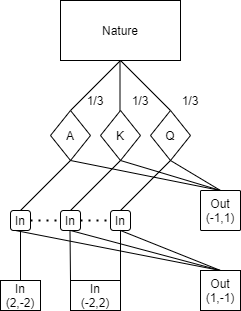
\includegraphics{diag}
\end{center}

The above sequential game formulation represents the game described. 
\subsection{Part B}
Player 1's pure strategy set is $\{in,out\}^3$. Player 2's pure strategy set is $\{in,out\}$.
\subsection{Part C}

If player 2 believes that player 1's card is an ace with probability 1, they will fold. If player 2 believes that player 1's card is a king or queen with probability 1, they  will fold. Let $p_A$ be the probability that player 1 drew an ace, given that they raised. Then, player 2 will call if $p_A(-2) + (1-p_A)(2)> -1\Rightarrow p_A< 3/4$. They would be indifferent between calling or not if $p_A = 3/4,$ and will fold if $p_A>3/4$. 

If player 1 draws an ace, they will receive 1 or 2 utility by calling, and -1 if they fold, so they will call. If they draw a card that is not an ace, they will recieve 1 utility by raising if they know the opponent will fold, but will lose 2 by calling if the opponent will fold. They will  always lose 1 utililty if they fold.

Player 1's optimal strategy is to always call if they draw an ace, and to also call on whatever proportion of non-aces will make player 2 indifferent between calling and folding. Player 2 will be indifferent if $p_A = 3/4$, so, with $\sigma_k,\sigma_q$ being the fraction of kings and queens that player 1 will call on, $3/4 = \frac{1/3}{1/3 + \sigma_k/3 +\sigma_q/3} \Rightarrow \sigma_k + \sigma_q = 1/3.$ 

Player 1 will only mix on a king or queen if they are indifferent: $-2\sigma_2 +(1-\sigma_2)1 = -1 \Rightarrow \sigma_2 = 2/3$. 

Therefore, Player 1's optimal strategy is to raise whenever they draw an ace, raise $(\sigma_k,\sigma_q) \in \{ (a,b)|(a,b) \in\mathbb{R}^2, a+b = 1/3 \} $ of the time whenever they draw a king or queen, and player 2's optimal strategy is to fold with probability $1/3$. Player 2 will believe that the card they are betting on is an ace with probability 3/4, king with probability $\sigma_k(3/4),$ and queen with probability $\sigma_q(3/4)$.
\end{document}
